\documentclass{standalone}
% analysis/style.tex — shared pgfplots preamble; % analysis/style.tex — shared pgfplots preamble; % analysis/style.tex — shared pgfplots preamble; \input{../style} from figures/
\usepackage[eulergreek]{sansmath}
\usepackage{pgfplots}
\usepackage{pgfplotstable}
\usepackage{xspace}

% Scheme-name macros — mirror the paper's meta/templates.tex so figure
% legends/titles/captions can write \plaintext / \sap / \emvp / \bntm /
% \tiptoe and render identically in both contexts. `\providecommand`
% lets the paper's templates.tex (loaded earlier) win when this file
% is in the paper as plots/pgfstyle.tex; in standalone artefact compiles
% these are the source of the macros.
\providecommand{\plaintext}{\textsc{Plaintext}\xspace}
\providecommand{\sap}{\textsc{SAP}\xspace}
\providecommand{\emvp}{\textsc{EMVP}\xspace}
\providecommand{\bntm}{\textsc{BNTM}\xspace}
\providecommand{\tiptoe}{\textsc{Tiptoe}\xspace}

\pgfplotsset{compat=newest}
\usepgfplotslibrary{units,colorbrewer,groupplots,fillbetween,statistics}
\usetikzlibrary{arrows.meta,backgrounds,calc,fit,shapes.geometric,positioning,patterns,shapes.misc}

% Bar charts request the colorbrewer Paired-12 cycle list directly via
% `cycle list/Paired-12` (loaded above by \usepgfplotslibrary{colorbrewer}).
% The library's `Paired-N` lists are full-colour, paper-quality, and live
% inside pgfplots so we don't ship a hand-rolled equivalent here.

\pgfplotsset{
  width=3.25in, height=2.5in,
  every axis/.append style={
    semithick,
    ymajorgrids=true,
    label style={font=\sffamily\small},
    title style={font=\sffamily\small},
  },
  % Line plots default to thick. `smooth` is NOT global — it is
  % opt-in per figure (added inside the axis options of figures 01,
  % 02, 04, 05, 06 that benefit from cubic interpolation). Putting
  % `smooth` in the global default fights pgfplots' `ybar` state
  % machine in figure 03 and `[only marks]` plots elsewhere; the
  % per-figure opt-in is cleaner than chasing local overrides.
  every axis plot/.append style={thick},
  legend style={
    draw=none,
    % Fully transparent legend container so overlap with plot title /
    % data points is visually obvious during figure tuning, rather
    % than silently masked. `fill=none` alone leaves an opaque white
    % rectangle on some pgfplots versions; pinning `fill opacity=0`
    % belt-and-braces guarantees see-through.
    fill=none,
    text opacity=1,
    anchor=south,
    at={(0.5,1)},
    font=\sffamily\small,
  },
  legend cell align=left,
  legend columns=-1,
  xtick align=outside,
  xtick pos=bottom,
  major tick length=1mm,
  tick label style={font=\sansmath\sffamily\small},
  every axis label={font=\sffamily\small},
  label style={font=\sffamily\small},
  {cycle list/Dark2},
  {cycle list/Set1},
  cycle list name=Dark2,
  cycle multiindex* list={
    Dark2\nextlist
    {solid,dashed,dotted,dashdotted,densely dashdotdotted}\nextlist
    mark list*\nextlist
  },
  /pgfplots/short line legend/.style={
    legend image code/.code={
      \draw[mark repeat=2,mark phase=2,##1]
        plot coordinates {(0cm,0cm)(0.2cm,0cm)(0.4cm,0cm)};
    }
  },
  /pgfplots/ybar legend/.style={
    /pgfplots/legend image code/.code={
      \draw[##1,/tikz/.cd,yshift=-0.25em](0cm,0cm) rectangle (4pt,6pt);
    },
  },
  /pgfplots/xbar legend/.style={
    /pgfplots/legend image code/.code={
      \draw[##1,/tikz/.cd,yshift=-0.25em](0cm,0cm) rectangle (4pt,6pt);
    },
  },
  select coords between index/.style 2 args={
    x filter/.code={
      \ifnum\coordindex<#1\def\pgfmathresult{}\fi
      \ifnum\coordindex>#2\def\pgfmathresult{}\fi
    }
  },
  discard if not/.style 2 args={
    x filter/.code={
      \edef\tempa{\thisrow{#1}}
      \edef\tempb{#2}
      \ifx\tempa\tempb
      \else
        \def\pgfmathresult{inf}
      \fi
    }
  },
}
 from figures/
\usepackage[eulergreek]{sansmath}
\usepackage{pgfplots}
\usepackage{pgfplotstable}
\usepackage{xspace}

% Scheme-name macros — mirror the paper's meta/templates.tex so figure
% legends/titles/captions can write \plaintext / \sap / \emvp / \bntm /
% \tiptoe and render identically in both contexts. `\providecommand`
% lets the paper's templates.tex (loaded earlier) win when this file
% is in the paper as plots/pgfstyle.tex; in standalone artefact compiles
% these are the source of the macros.
\providecommand{\plaintext}{\textsc{Plaintext}\xspace}
\providecommand{\sap}{\textsc{SAP}\xspace}
\providecommand{\emvp}{\textsc{EMVP}\xspace}
\providecommand{\bntm}{\textsc{BNTM}\xspace}
\providecommand{\tiptoe}{\textsc{Tiptoe}\xspace}

\pgfplotsset{compat=newest}
\usepgfplotslibrary{units,colorbrewer,groupplots,fillbetween,statistics}
\usetikzlibrary{arrows.meta,backgrounds,calc,fit,shapes.geometric,positioning,patterns,shapes.misc}

% Bar charts request the colorbrewer Paired-12 cycle list directly via
% `cycle list/Paired-12` (loaded above by \usepgfplotslibrary{colorbrewer}).
% The library's `Paired-N` lists are full-colour, paper-quality, and live
% inside pgfplots so we don't ship a hand-rolled equivalent here.

\pgfplotsset{
  width=3.25in, height=2.5in,
  every axis/.append style={
    semithick,
    ymajorgrids=true,
    label style={font=\sffamily\small},
    title style={font=\sffamily\small},
  },
  % Line plots default to thick. `smooth` is NOT global — it is
  % opt-in per figure (added inside the axis options of figures 01,
  % 02, 04, 05, 06 that benefit from cubic interpolation). Putting
  % `smooth` in the global default fights pgfplots' `ybar` state
  % machine in figure 03 and `[only marks]` plots elsewhere; the
  % per-figure opt-in is cleaner than chasing local overrides.
  every axis plot/.append style={thick},
  legend style={
    draw=none,
    % Fully transparent legend container so overlap with plot title /
    % data points is visually obvious during figure tuning, rather
    % than silently masked. `fill=none` alone leaves an opaque white
    % rectangle on some pgfplots versions; pinning `fill opacity=0`
    % belt-and-braces guarantees see-through.
    fill=none,
    text opacity=1,
    anchor=south,
    at={(0.5,1)},
    font=\sffamily\small,
  },
  legend cell align=left,
  legend columns=-1,
  xtick align=outside,
  xtick pos=bottom,
  major tick length=1mm,
  tick label style={font=\sansmath\sffamily\small},
  every axis label={font=\sffamily\small},
  label style={font=\sffamily\small},
  {cycle list/Dark2},
  {cycle list/Set1},
  cycle list name=Dark2,
  cycle multiindex* list={
    Dark2\nextlist
    {solid,dashed,dotted,dashdotted,densely dashdotdotted}\nextlist
    mark list*\nextlist
  },
  /pgfplots/short line legend/.style={
    legend image code/.code={
      \draw[mark repeat=2,mark phase=2,##1]
        plot coordinates {(0cm,0cm)(0.2cm,0cm)(0.4cm,0cm)};
    }
  },
  /pgfplots/ybar legend/.style={
    /pgfplots/legend image code/.code={
      \draw[##1,/tikz/.cd,yshift=-0.25em](0cm,0cm) rectangle (4pt,6pt);
    },
  },
  /pgfplots/xbar legend/.style={
    /pgfplots/legend image code/.code={
      \draw[##1,/tikz/.cd,yshift=-0.25em](0cm,0cm) rectangle (4pt,6pt);
    },
  },
  select coords between index/.style 2 args={
    x filter/.code={
      \ifnum\coordindex<#1\def\pgfmathresult{}\fi
      \ifnum\coordindex>#2\def\pgfmathresult{}\fi
    }
  },
  discard if not/.style 2 args={
    x filter/.code={
      \edef\tempa{\thisrow{#1}}
      \edef\tempb{#2}
      \ifx\tempa\tempb
      \else
        \def\pgfmathresult{inf}
      \fi
    }
  },
}
 from figures/
\usepackage[eulergreek]{sansmath}
\usepackage{pgfplots}
\usepackage{pgfplotstable}
\usepackage{xspace}

% Scheme-name macros — mirror the paper's meta/templates.tex so figure
% legends/titles/captions can write \plaintext / \sap / \emvp / \bntm /
% \tiptoe and render identically in both contexts. `\providecommand`
% lets the paper's templates.tex (loaded earlier) win when this file
% is in the paper as plots/pgfstyle.tex; in standalone artefact compiles
% these are the source of the macros.
\providecommand{\plaintext}{\textsc{Plaintext}\xspace}
\providecommand{\sap}{\textsc{SAP}\xspace}
\providecommand{\emvp}{\textsc{EMVP}\xspace}
\providecommand{\bntm}{\textsc{BNTM}\xspace}
\providecommand{\tiptoe}{\textsc{Tiptoe}\xspace}

\pgfplotsset{compat=newest}
\usepgfplotslibrary{units,colorbrewer,groupplots,fillbetween,statistics}
\usetikzlibrary{arrows.meta,backgrounds,calc,fit,shapes.geometric,positioning,patterns,shapes.misc}

% Bar charts request the colorbrewer Paired-12 cycle list directly via
% `cycle list/Paired-12` (loaded above by \usepgfplotslibrary{colorbrewer}).
% The library's `Paired-N` lists are full-colour, paper-quality, and live
% inside pgfplots so we don't ship a hand-rolled equivalent here.

\pgfplotsset{
  width=3.25in, height=2.5in,
  every axis/.append style={
    semithick,
    ymajorgrids=true,
    label style={font=\sffamily\small},
    title style={font=\sffamily\small},
  },
  % Line plots default to thick. `smooth` is NOT global — it is
  % opt-in per figure (added inside the axis options of figures 01,
  % 02, 04, 05, 06 that benefit from cubic interpolation). Putting
  % `smooth` in the global default fights pgfplots' `ybar` state
  % machine in figure 03 and `[only marks]` plots elsewhere; the
  % per-figure opt-in is cleaner than chasing local overrides.
  every axis plot/.append style={thick},
  legend style={
    draw=none,
    % Fully transparent legend container so overlap with plot title /
    % data points is visually obvious during figure tuning, rather
    % than silently masked. `fill=none` alone leaves an opaque white
    % rectangle on some pgfplots versions; pinning `fill opacity=0`
    % belt-and-braces guarantees see-through.
    fill=none,
    text opacity=1,
    anchor=south,
    at={(0.5,1)},
    font=\sffamily\small,
  },
  legend cell align=left,
  legend columns=-1,
  xtick align=outside,
  xtick pos=bottom,
  major tick length=1mm,
  tick label style={font=\sansmath\sffamily\small},
  every axis label={font=\sffamily\small},
  label style={font=\sffamily\small},
  {cycle list/Dark2},
  {cycle list/Set1},
  cycle list name=Dark2,
  cycle multiindex* list={
    Dark2\nextlist
    {solid,dashed,dotted,dashdotted,densely dashdotdotted}\nextlist
    mark list*\nextlist
  },
  /pgfplots/short line legend/.style={
    legend image code/.code={
      \draw[mark repeat=2,mark phase=2,##1]
        plot coordinates {(0cm,0cm)(0.2cm,0cm)(0.4cm,0cm)};
    }
  },
  /pgfplots/ybar legend/.style={
    /pgfplots/legend image code/.code={
      \draw[##1,/tikz/.cd,yshift=-0.25em](0cm,0cm) rectangle (4pt,6pt);
    },
  },
  /pgfplots/xbar legend/.style={
    /pgfplots/legend image code/.code={
      \draw[##1,/tikz/.cd,yshift=-0.25em](0cm,0cm) rectangle (4pt,6pt);
    },
  },
  select coords between index/.style 2 args={
    x filter/.code={
      \ifnum\coordindex<#1\def\pgfmathresult{}\fi
      \ifnum\coordindex>#2\def\pgfmathresult{}\fi
    }
  },
  discard if not/.style 2 args={
    x filter/.code={
      \edef\tempa{\thisrow{#1}}
      \edef\tempb{#2}
      \ifx\tempa\tempb
      \else
        \def\pgfmathresult{inf}
      \fi
    }
  },
}

\providecommand{\datadir}{../data}
\begin{document}
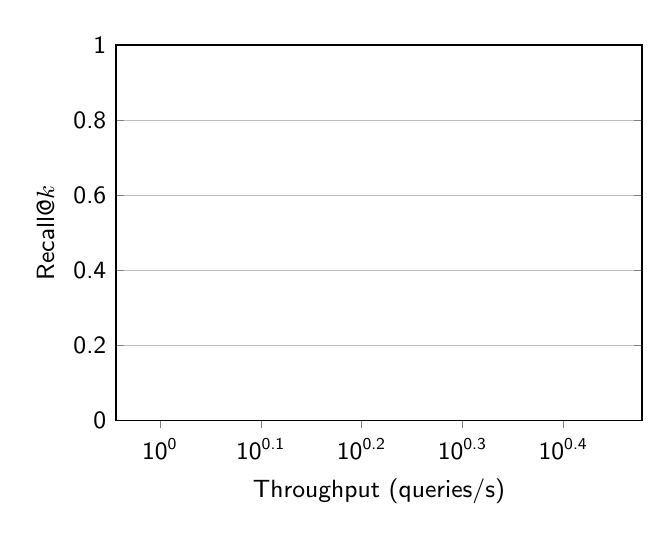
\begin{tikzpicture}
  \begin{axis}[
    % Figure 11. Same axes as figure 02 (recall vs QPS,
    % log-x), but each scheme contributes two lines: CPU solid and
    % GPU dashed of the same colour. \tiptoe is dotted because its
    % GPU number is the analytical proxy only.
    xlabel={Throughput (queries/s)},
    ylabel={Recall@$k$},
    xmode=log,
    ymin=0, ymax=1,
    every axis plot/.append style={
      smooth,
      error bars/x dir=both,
      error bars/x explicit,
    },
    legend columns=3,
    % `unbounded coords=jump` lets pgfplots tolerate `nan` cells when
    % a scheme is measured on only one substrate (the emitter writes
    % `nan` for the missing column).
    unbounded coords=jump,
    cycle list name=Set1,
  ]
    % \plaintext: CPU solid, GPU dashed of the same colour. Cycling
    % the colour list per pair (cycle list shift=1 across the
    % subsequent solid/dashed sets) keeps each scheme's CPU/GPU
    % share a single colour entry. The shared-colour pattern is
    % expressed by repeating the cycle: pgfplots advances the
    % cycle on each \addplot, so we use \pgfplotsset{cycle list shift}
    % implicitly via the order of legend entries — `\plaintext (CPU)`
    % and `\plaintext (GPU)` are entries 0 and 1, but the colour
    % the eye reads is the same because we set `mark=none` on GPU
    % lines and rely on `dashed` to disambiguate.
    \IfFileExists{\datadir/recall-throughput-cpu-vs-gpu-plaintext.tsv}{
      \addplot+[mark=*] table[col sep=tab, x=qps_cpu, x error=qps_cpu_rep_ci95,
                              y=recall_mean_cpu]
        {\datadir/recall-throughput-cpu-vs-gpu-plaintext.tsv};
      \addlegendentry{\plaintext CPU}
      \addplot+[mark=*, dashed] table[col sep=tab, x=qps_gpu,
                                       x error=qps_gpu_rep_ci95,
                                       y=recall_mean_gpu]
        {\datadir/recall-throughput-cpu-vs-gpu-plaintext.tsv};
      \addlegendentry{\plaintext GPU}
    }{}
    \IfFileExists{\datadir/recall-throughput-cpu-vs-gpu-sap-ivf-nprobe.tsv}{
      \addplot+[mark=square*] table[col sep=tab, x=qps_cpu,
                                     x error=qps_cpu_rep_ci95,
                                     y=recall_mean_cpu]
        {\datadir/recall-throughput-cpu-vs-gpu-sap-ivf-nprobe.tsv};
      \addlegendentry{\sap+IVF CPU}
      \addplot+[mark=square*, dashed] table[col sep=tab, x=qps_gpu,
                                             x error=qps_gpu_rep_ci95,
                                             y=recall_mean_gpu]
        {\datadir/recall-throughput-cpu-vs-gpu-sap-ivf-nprobe.tsv};
      \addlegendentry{\sap+IVF GPU}
    }{}
    \IfFileExists{\datadir/recall-throughput-cpu-vs-gpu-emvp-ivf-nprobe.tsv}{
      \addplot+[mark=triangle*] table[col sep=tab, x=qps_cpu,
                                       x error=qps_cpu_rep_ci95,
                                       y=recall_mean_cpu]
        {\datadir/recall-throughput-cpu-vs-gpu-emvp-ivf-nprobe.tsv};
      \addlegendentry{\emvp+IVF CPU}
      \addplot+[mark=triangle*, dashed] table[col sep=tab, x=qps_gpu,
                                               x error=qps_gpu_rep_ci95,
                                               y=recall_mean_gpu]
        {\datadir/recall-throughput-cpu-vs-gpu-emvp-ivf-nprobe.tsv};
      \addlegendentry{\emvp+IVF GPU}
    }{}
    \IfFileExists{\datadir/recall-throughput-cpu-vs-gpu-bntm-ivf-nprobe.tsv}{
      \addplot+[mark=diamond*] table[col sep=tab, x=qps_cpu,
                                      x error=qps_cpu_rep_ci95,
                                      y=recall_mean_cpu]
        {\datadir/recall-throughput-cpu-vs-gpu-bntm-ivf-nprobe.tsv};
      \addlegendentry{\bntm+IVF CPU}
      \addplot+[mark=diamond*, dashed] table[col sep=tab, x=qps_gpu,
                                              x error=qps_gpu_rep_ci95,
                                              y=recall_mean_gpu]
        {\datadir/recall-throughput-cpu-vs-gpu-bntm-ivf-nprobe.tsv};
      \addlegendentry{\bntm+IVF GPU}
    }{}
    % \tiptoe-GPU is the analytical proxy only — no
    % measured GPU line. The CPU line is what the existing figure 02
    % already shows; we omit the dotted-GPU projection from this
    % chart and let figure 12 (effective bytes) carry the proxy.
    \IfFileExists{\datadir/recall-throughput-tiptoe.tsv}{
      \addplot+[mark=o, densely dotted] table[col sep=tab, x=qps,
                                                x error=qps_rep_ci95,
                                                y=recall_mean]
        {\datadir/recall-throughput-tiptoe.tsv};
      \addlegendentry{\tiptoe CPU}
    }{}
  \end{axis}
\end{tikzpicture}
\end{document}
